% ------------------------------------------------------------------------------
% TYPO3 CMS 7.3 - What's New - Chapter "Extbase & Fluid" (English Version)
%
% @author	Michael Schams <schams.net>
% @license	Creative Commons BY-NC-SA 3.0
% @link		http://typo3.org/download/release-notes/whats-new/
% @language	English
% ------------------------------------------------------------------------------
% LTXE-CHAPTER-UID:		ba9bf9d9-564d719b-a45c6394-358e2ef2
% LTXE-CHAPTER-NAME:	Chapter: Extbase & Fluid
% ------------------------------------------------------------------------------

\section{Extbase и Fluid}
\begin{frame}[fragile]
	\frametitle{Extbase и Fluid}

	\begin{center}\huge{Глава 4:}\end{center}
	\begin{center}\huge{\color{typo3darkgrey}\textbf{Extbase и Fluid}}\end{center}

\end{frame}

% ------------------------------------------------------------------------------
% LTXE-SLIDE-START
% LTXE-SLIDE-UID:		2e2161ff-12d25de3-4c0001f8-eb3e58f3
% LTXE-SLIDE-ORIGIN:	5d89ef1b-822aec7b-91faf04c-562236d0 English
% LTXE-SLIDE-ORIGIN:	b5ee213c-b04df592-d31ed084-b94e0f58 German
% LTXE-SLIDE-TITLE:		Feature #62242: ActionMenuItemGroupViewHelper (1)
% LTXE-SLIDE-REFERENCE:	Feature-62242-ActionMenuItemGroupViewHelper.rst
% ------------------------------------------------------------------------------

\begin{frame}[fragile]
	\frametitle{Extbase и Fluid}
	\framesubtitle{ActionMenuItemGroupViewHelper (1)}

	% decrease font size for code listing
	\lstset{basicstyle=\tiny\ttfamily}

	\begin{itemize}

		\item Этот проектор/ViewHelper позволяет использовать группы параметров в полях выбора внутреннего интерфейса,
			контролирующие выбираемые действия

		\item Пример:
			\begin{lstlisting}
				<f:be.menus.actionMenu>
				  <f:be.menus.actionMenuItem label="Default: Welcome" controller="Default" action="index" />
				  <f:be.menus.actionMenuItem label="Community: get in touch" controller="Community"
				    action="index" />
				  <f:be.menus.actionMenuItemGroup label="Information">
				    <f:be.menus.actionMenuItem label="PHP Information" controller="Information"
				      action="listPhpInfo" />
				    <f:be.menus.actionMenuItem label="Documentation" controller="Information"
				      action="documentation" />
				    <f:be.menus.actionMenuItem label="Hooks" controller="Information" action="hooks" />
				    <f:be.menus.actionMenuItem label="Signals" controller="Information" action="signals" />
				    <f:be.menus.actionMenuItem label="XClasses" controller="Information" action="xclass" />
				  </f:be.menus.actionMenuItemGroup>
				</f:be.menus.actionMenu>
			\end{lstlisting}

	\end{itemize}

\end{frame}

% ------------------------------------------------------------------------------
% LTXE-SLIDE-START
% LTXE-SLIDE-UID:		8a12aa72-269daabe-21c6d364-7204ca6a
% LTXE-SLIDE-ORIGIN:	c5a36e6f-c177e6e6-18628419-eaf4b653 English
% LTXE-SLIDE-ORIGIN:	b04df592-d31ed084-b94e0f58-b5ee213c German
% LTXE-SLIDE-TITLE:		Feature #62242: ActionMenuItemGroupViewHelper (2)
% LTXE-SLIDE-REFERENCE:	Feature-62242-ActionMenuItemGroupViewHelper.rst
% ------------------------------------------------------------------------------

\begin{frame}[fragile]
	\frametitle{Extbase и Fluid}
	\framesubtitle{ActionMenuItemGroupViewHelper (2)}

	\begin{itemize}
		\item Пример предыдущего слайда выводится следующим образом:
	\end{itemize}

	\begin{figure}
		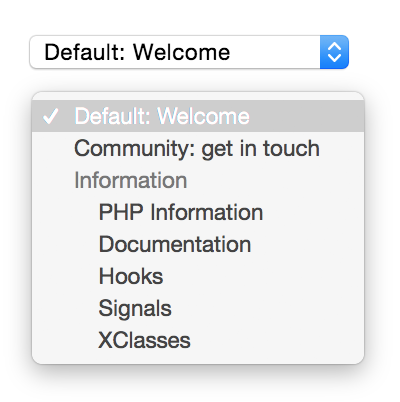
\includegraphics[width=0.3\linewidth]{ExtbaseFluid/62242.png}
	\end{figure}

\end{frame}

% ------------------------------------------------------------------------------
% LTXE-SLIDE-START
% LTXE-SLIDE-UID:		d09960b8-b3e4915f-c8e64993-53fe45bc
% LTXE-SLIDE-ORIGIN:	ea102c24-20cdb8de-eb67260a-af2a6967 English
% LTXE-SLIDE-ORIGIN:	44467f9a-abe64946-3da2bf4c-5bd094eb German
% LTXE-SLIDE-TITLE:		Feature/Breaking #63453: Template support for FlashMessagesViewHelper
% LTXE-SLIDE-REFERENCE:	Feature-63453-TemplateSupportForFlashMessagesViewHelper.rst
% LTXE-SLIDE-REFERENCE:	Breaking-63453-ChangedRenderingOfFlashMessagesViewHelper.rst
% ------------------------------------------------------------------------------

\begin{frame}[fragile]
	\frametitle{Extbase и Fluid}
	\framesubtitle{Поддержка шаблонов для FlashMessagesViewHelper}

	% decrease font size for code listing
	\lstset{basicstyle=\tiny\ttfamily}

	\begin{itemize}

		\item Теперь \texttt{FlashMessagesViewHelper} поддерживает шаблоны/templates

		\item Новый атрибут \texttt{as} позволяет указать название переменной, которую можно использовать
			внутри дочерних элементов проектора/ViewHelper для доступа к всплывающим сообщениям

		\item Пример:

			\begin{lstlisting}
				<f:flashMessages as="flashMessages">
				  <ul class="myFlashMessages">
				    <f:for each="{flashMessages}" as="flashMessage">
				      <li class="alert {flashMessage.class}">
				        <h4>{flashMessage.title}</h4>
				        <span class="fancy-icon">{flashMessage.message}</span>
				      </li>
				    </f:for>
				  </ul>
				</f:flashMessages>
			\end{lstlisting}

		\item Замечание: теперь параметр \texttt{renderMode} устарел

	\end{itemize}

\end{frame}

% ------------------------------------------------------------------------------
% LTXE-SLIDE-START
% LTXE-SLIDE-UID:		64153520-a7354104-753da80d-b8ffe0b7
% LTXE-SLIDE-ORIGIN:	3f5a8c27-78ff086f-99844ec0-a5e2d74a English
% LTXE-SLIDE-ORIGIN:	ec0810a7-c987f58a-9c42904e-8b7e0eba German
% LTXE-SLIDE-TITLE:		Feature #66111: Add TemplateRootPaths support to cObject FLUIDTEMPLATE (1)
% LTXE-SLIDE-REFERENCE:	Feature-66111-AddTemplaterootpathsSupportToCobjectFluidtemplate.rst
% ------------------------------------------------------------------------------

\begin{frame}[fragile]
	\frametitle{Extbase и Fluid}
	\framesubtitle{Новые свойства cObject \texttt{FLUIDTEMPLATE} (1)}

	\begin{itemize}

		\item cObject \texttt{FLUIDTEMPLATE} был дополнен
			\texttt{templateRootPaths} и \texttt{templateName}

		\item Что позволяет указать название шаблона и для вывода будет использован
			шаблон с этим названием наряду с указанным форматом по пути для шаблонов из настройки
			\texttt{templateRootPaths}

		\item \texttt{templateRootPaths} использует ту же логику резервирования, что и 
			\texttt{layoutRootPath} и \texttt{partialRootPath}

			\begin{itemize}
				\item templateName: string/stdWrap
				\item templateRootPaths: массив путей к файлам с поддержкой префикса "EXT:"
			\end{itemize}

	\end{itemize}

\end{frame}

% ------------------------------------------------------------------------------
% LTXE-SLIDE-START
% LTXE-SLIDE-UID:		017f8145-53121ac0-c8f39a46-2cda72f7
% LTXE-SLIDE-ORIGIN:	90d6213a-883bc8d8-9c60e454-fac818a6 English
% LTXE-SLIDE-ORIGIN:	ec0810a7-c987f58a-9c42904e-8b7e0eba German
% LTXE-SLIDE-TITLE:		Feature #66111: Add TemplateRootPaths support to cObject FLUIDTEMPLATE (2)
% LTXE-SLIDE-REFERENCE:	Feature-66111-AddTemplaterootpathsSupportToCobjectFluidtemplate.rst
% ------------------------------------------------------------------------------

\begin{frame}[fragile]
	\frametitle{Extbase и Fluid}
	\framesubtitle{Новые свойства cObject \texttt{FLUIDTEMPLATE} (2)}

	% decrease font size for code listing
	\lstset{basicstyle=\tiny\ttfamily}

	\begin{itemize}

		\item Пример TypoScript:

			\begin{lstlisting}
				lib.stdContent = FLUIDTEMPLATE
				lib.stdContent {
				  templateName = TEXT
				  templateName.stdWrap {
				    cObject = TEXT
				    cObject {
				      data = levelfield:-2,backend_layout_next_level,slide
				      override.field = backend_layout
				      split {
				        token = frontend__
				        1.current = 1
				        1.wrap = |
				      }
				    }
				    ifEmpty = Default
				  }
				  templateRootPaths {
				    10 = EXT:frontend/Resources/Private/Templates
				    20 = EXT:sitemodification/Resources/Private/Templates
				  }
				}
			\end{lstlisting}

	\end{itemize}

\end{frame}

% ------------------------------------------------------------------------------
% LTXE-SLIDE-START
% LTXE-SLIDE-UID:		8bbaac30-f8def338-24fd5a98-ffd78d34
% LTXE-SLIDE-ORIGIN:	227004ec-e3e23728-e01cd083-cab72f98 English
% LTXE-SLIDE-ORIGIN:	5d3c259c-f79dd1fe-4f272783-a63cf715 German
% LTXE-SLIDE-TITLE:		Feature #66269: Fluid: Remove ViewHelper xmlns-attributes and specified html tag (1)
% LTXE-SLIDE-REFERENCE:	Feature-66269-FluidRemoveViewHelperXmlnsAttributesAndSpecifiedHtmlTag.rst
% ------------------------------------------------------------------------------

\begin{frame}[fragile]
	\frametitle{Extbase и Fluid}
	\framesubtitle{Удаление \texttt{xmlns}-атрибутов и тегов HTML (1)}

	% decrease font size for code listing
	\lstset{basicstyle=\tiny\ttfamily}

	\begin{itemize}

		\item С введенем в обиход атрибутов \texttt{xmlns:*} для подключения
			проекторов/ViewHelpers, стала возможна поддержка со стороны IDE для шаблонов Fluid.
			Проблема была в том, что атрибуты \texttt{xmlns:*} с соответствующим тегом
			также выводились, что обычно нежелательно.

		\item Обойти проблему удавалось с использованием  sections, но такое решение неинтуитивно понятно,
			и недопустимо в макетах/layouts. Это также негативно отражается на задействованных ресурсах.

		\item \texttt{xmlns:*} атрибуты для верных областей именования ViewHelper теперь удаляются перед выводом,
			если используется следующий синтаксис:
			\small\texttt{http://typo3.org/ns/<phpNamespace>}\normalsize\newline
			(\texttt{xmlns} атрибуты для не-ViewHelper областей — сохраняются)

	\end{itemize}

\end{frame}

% ------------------------------------------------------------------------------
% LTXE-SLIDE-START
% LTXE-SLIDE-UID:		aa14c458-8291959c-6856660e-5a8aa070
% LTXE-SLIDE-ORIGIN:	78a19608-9b89498f-d9a26bb5-11fb53c8 English
% LTXE-SLIDE-ORIGIN:	27834f27-5d3c259c-f79dd1fe-a63cf715 German
% LTXE-SLIDE-TITLE:		Feature #66269: Fluid: Remove ViewHelper xmlns-attributes and specified html tag (2)
% LTXE-SLIDE-REFERENCE:	Feature-66269-FluidRemoveViewHelperXmlnsAttributesAndSpecifiedHtmlTag.rst
% ------------------------------------------------------------------------------

\begin{frame}[fragile]
	\frametitle{Extbase и Fluid}
	\framesubtitle{Удаление \texttt{xmlns}-атрибутов и тегов HTML (2)}

	% decrease font size for code listing
	\lstset{basicstyle=\tiny\ttfamily}

	\begin{itemize}

		\item Включение областей именования ViewHelper внутри тега HTML с атрибутом
			\texttt{data-namespace-typo3-fluid="true"} для предотвращения вывода
			всего тега HTML

			\begin{lstlisting}
				<html data-namespace-typo3-fluid="true"
				  xmlns:f="http://typo3.org/ns/TYPO3/CMS/Fluid/ViewHelpers"
				  xmlns:n="http://typo3.org/ns/GeorgRinger/News/ViewHelpers">

				  <f:if condition="{newsItem.title}">
				    <f:then>
				      <n:titleTag>{newsItem.title}</n:titleTag>
				    </f:then>
				    <f:else>
				      <n:titleTag>News-Detail</n:titleTag>
				    </f:else>
				  </f:if>

				</html>
			\end{lstlisting}

	\end{itemize}

\end{frame}

% ------------------------------------------------------------------------------
% LTXE-SLIDE-START
% LTXE-SLIDE-UID:		e46d6de8-d11c64a6-5fddb9be-7cae8add
% LTXE-SLIDE-ORIGIN:	a1ef516c-669ded34-a2a6d664-f4d82d94 English
% LTXE-SLIDE-ORIGIN:	f79dd1fe-4f272783-a63cf715-5d3c259c German
% LTXE-SLIDE-TITLE:		Feature #66709: Add TemplateRootPaths support to Fluid/View/StandaloneView
% LTXE-SLIDE-REFERENCE:	Feature-66709-AddTemplateRootPathsSupportToFluidViewStandaloneView.rst
% ------------------------------------------------------------------------------

\begin{frame}[fragile]
	\frametitle{Extbase и Fluid}
	\framesubtitle{Новые методы во Fluid-StandaloneView}

	% decrease font size for code listing
	\lstset{basicstyle=\tiny\ttfamily}

	\begin{itemize}

		\item StandaloneView дополнен
			\texttt{setTemplateRootPaths(\$templatePaths)} и
			\texttt{setTemplate(\$templateName, \$throwException = TRUE)}

		\item с тем же функционалом, что и cObject \texttt{FLUIDTEMPLATE}

		\item Пример (вывод шаблона email):

			\begin{lstlisting}
				$view = GeneralUtility::makeInstance(StandaloneView::class);
				$view->setLayoutRootPaths(array(GeneralUtility::getFileAbsFileName(
				  'EXT:my_extension/Resources/Private/Layouts')));
				$view->setPartialRootPaths(array(GeneralUtility::getFileAbsFileName(
				  'EXT:my_extension/Resources/Private/Partials')));
				$view->setTemplateRootPaths(array(GeneralUtility::getFileAbsFileName(
				  'EXT:my_extension/Resources/Private/Templates')));
				$view->setTemplate('Email/Notification');
				$emailBody = $view->render();
			\end{lstlisting}

	\end{itemize}

\end{frame}

% ------------------------------------------------------------------------------
% LTXE-SLIDE-START
% LTXE-SLIDE-UID:		d097ac3b-f9a4d4e3-10d393b7-918a11b4
% LTXE-SLIDE-ORIGIN:	95baf76c-31fd3f59-e0f9a716-5a5cc8cb English
% LTXE-SLIDE-ORIGIN:	f79da63cf-7834f272-d1fe715-5d3c259c German
% LTXE-SLIDE-TITLE:		Feature #66907: Add Data Processing to FLUIDTEMPLATE content object (1)
% LTXE-SLIDE-REFERENCE:	Feature-66907-AddDataProcessingToFluidTemplateContentObject.rst
% ------------------------------------------------------------------------------

\begin{frame}[fragile]
	\frametitle{Extbase и Fluid}
	\framesubtitle{Обработка данных для \texttt{FLUIDTEMPLATE} cObject (1)}

	% decrease font size for code listing
	\lstset{basicstyle=\smaller\ttfamily}

	\begin{itemize}

		\item cObject \texttt{FLUIDTEMPLATE} дополнен \texttt{dataProcessing}

		\item Эта настройка служит для добавления одного или нескольких обработчиков для
			работы с переменной \texttt{\$data} выводимого в текущий момент cObject\newline
			(например, \texttt{tt\_content} или \texttt{page})

		\item Процессор должен реализовывать интерфейс
			\texttt{FluidTemplateDataProcessorInterface} и содержать следующий метод:

			\begin{lstlisting}
				function process(array &$data, array $processorConfiguration,
				  array $configuration, StandaloneView $view) {
				    [...]
				}
			\end{lstlisting}

	\end{itemize}

\end{frame}

% ------------------------------------------------------------------------------
% LTXE-SLIDE-START
% LTXE-SLIDE-UID:		1dcc8570-8f84e662-71354a70-234b9b34
% LTXE-SLIDE-ORIGIN:	34ef94b7-988b06b4-78e81c3a-81e45590 English
% LTXE-SLIDE-ORIGIN:	4f272783-a63cf715-5d3c259c-f79dd1fe German
% LTXE-SLIDE-TITLE:		Feature #66907: Add Data Processing to FLUIDTEMPLATE content object (2)
% LTXE-SLIDE-REFERENCE:	Feature-66907-AddDataProcessingToFluidTemplateContentObject.rst
% ------------------------------------------------------------------------------

\begin{frame}[fragile]
	\frametitle{Extbase и Fluid}
	\framesubtitle{Обработка данных для \texttt{FLUIDTEMPLATE} cObject (2)}

	% decrease font size for code listing
	\lstset{basicstyle=\tiny\ttfamily}

	\begin{itemize}

		\item Пример:

			\begin{lstlisting}
				my_custom_ctype = FLUIDTEMPLATE
				my_custom_ctype {
				  templateRootPaths {
				    10 = EXT:your_extension_key/Resources/Private/Templates
				  }
				  templateName = CustomName
				  settings {
				    extraParam = 1
				  }
				  dataProcessing {
				    1 = Vendor\YourExtensionKey\DataProcessing\MyFirstCustomProcessor
				    2 = AnotherVendor\AnotherExtensionKey\DataProcessing\MySecondCustomProcessor
				    2 {
				      options {
				        myOption = SomeValue
				      }
				    }
				  }
				}
			\end{lstlisting}

	\end{itemize}

\end{frame}

% ------------------------------------------------------------------------------
